\chapter{Auswertung und Vergleich mit Property-based Testing}
\label{experimente}

\section{Vergleichmetriken}

Bevor ein Vergleich beider Methoden durchgeführt werden kann, müssen erst einmal Metriken eingeführt werden, in denen sich verglichen werden soll.
Im Fokus des Vergleichs stehen die in \textit{Property-based Testing}~\cite{property-based-testing} genutzten Metriken.

\subsection{Metriken aus Property-based Testing}

In \textit{Property-based Testing} wurden zwei Metriken eingeführt, um die Methode zu evaluieren.
Es wurden zwei Forschungsfragen vorgestellt.

\begin{enumerate}
    \item Welche Schema Coverage kann mit der Methode erreicht werden?~\cite[vgl. RQ1]{property-based-testing}
    \item Wie gut ist die Fehlerfindungskapazität der Methode?~\cite[vgl. RQ2]{property-based-testing}
\end{enumerate}

Zur Beantwortung der Fragen wurden Experimente auf zwei Testsystemen ausgeführt.
Das erste Testsystem ist eine eigens entwickelte GraphQL-API, die bekannte Fehler besitzt~\cite[vgl. A.1]{property-based-testing}.
Testsystem zwei ist GitLab, eine häufig genutzte Software für GitServer mit DevOps Kapazitäten.
Gitlab bietet seine API auch als GraphQL an und durch seine riesige Größe eignet sich GitLab als solides Testsystem~\cite[vgl. A2]{property-based-testing}.
Der hier entwickelte Prototyp soll in exakt dem gleichen Umfeld seine Tests generieren.
Es ist zu erwarten, dass die selben Fehler gefunden werden wie in der Methode des \textit{Property-based Testings}.
Ideal wäre es, neue Fehler zu finden.
Beide Forschungsfragen werden im Folgenden noch einmal näher erläutert, da diese speziell sind und Wissen über die Methode wichtig ist, um die Ergebnisse korrekt einordnen zu können.

\subsection{Fehlerfindungskapazität}

Die Fehlerfindungskapazität ist eine Metrik, die messen soll, wie zuverlässig die Methode tatsächlich Fehler findet.
Hierfür werden die beiden zuvor benannten APIs getestet und es wird geprüft, ob die Methode die Fehler finden konnte.
Um zu verifizieren, dass die Methode möglichst viele Fehler findet, wurde eine Test API entwickelt, die mit bekannten Fehlern versehen wird.
Der Prototyp des \textit{Property-based Testing} fand 11 von 15 Fehlern im speziell vorbereiteten System.
Bei GitLab wurden 4 Bugs im Query-Bereich gefunden.
Der hier entwickelte Prototyp soll mindestens die gleichen Fehler finden und idealerweise mehr.

\subsection{GraphQL-Schema Abdeckung}
\label{propiskant}

Dadurch, dass \textit{Property-based Testing} auf zufallsbasierter Testgenerierung basiert, stellt sich die Frage, wie gut die Methode
die API abdeckt und inwiefern die generierten Tests ausreichend sind.
Dies kommt insbesondere zu tragen, wenn die maximale Pfadlänge ausgehend vom Query-Knoten größer ist als die erlaubte Rekursionstiefe des Prototypens.
In Property-based Testing wird definiert, dass die generierten Tests eine vollständige Abdeckung erreichen, wenn Definition~\ref{defedgecov} gilt.
Definition~\ref{defedgecov} entspricht im Allgemeinen der Kantenabdeckung nach Definition~\ref{edgecov}.

\begin{definition}
    Für alle Objekte des Schemas: Bilde alle Tupel \{Object, Field \}.
    Ein Schema hat eine ideale Coverage, wenn alle Tupel durch einen Test abgedeckt sind~\cite[vgl. B. Measuring Schema Coverage]{property-based-testing}.
    \label{defedgecov}
\end{definition}

Es sei erwähnt, dass die hier angesprochene Abdeckung eine theoretische Abdeckung ist.
Die tatsächlich erreichte Abdeckung wird nicht betrachtet.

\section{Threats to Validity / Limitierungen}

Bevor der eigentliche Vergleich beginnt, soll eingeordnet werden, inwiefern die Experimente zu betrachten sind.
Es wird gezeigt, welche Voraussetzungen nötig sind, um die hier erzielten Ergebnisse zu erlangen.

\subsection{Argumentgeneratoren}

Wie in Kapitel~\ref{zufallsgen} erwähnt, ist es wichtig, dass GraphQL für jede Funktion einen Wert ungleich $null$ liefert,
damit der Pfad weitergegangen werden kann und die Funktionen in diesem getestet werden, um die tatsächliche Abdeckung zu erhöhen.
Um die Wahrscheinlichkeit zu erhöhen, dass Argumentgeneratoren ein Argument zurückliefern, dass zum SUT passt, wurden diese angepasst.
Dabei wird die Vergleichbarkeit der Arbeiten nicht verletzt, da diese Anpassungen der Argumentgeneratoren in~\cite{property-based-testing} auch vorgenommen wurden \cite[vgl. Experimental Setup and Method]{property-based-testing}.
Hierbei sei zum Beispiel erwähnt, dass eine Type $ID$ in GraphQL als String wert definiert ist, häufig in Implementierung jedoch als Zahlenstring genutzt wird.
Eine Anpassung ist, dass der Generator, für den Type $ID$ so angepasst wird, dass er nur Argumente für $ID$ zurückliefert, die ein Zahlenstring sind.

\section{Fehlerfindungskapazitäten}

Zuerst soll die Fehlerfindungskapazität des Prototypens bewiesen werden.
Dafür werden die beiden zuvor benannten Testsysteme GraphQL-Toy~\ref{graphql-toy-code} und GitLab in der Version 12.6.3 verwendet.
Ziel ist es mindestens die Fehler zu finden, die vom \textit{Property-based Testtool}~\cite{property-based-testing} gefunden wurden.

\subsection{GraphQL-Toy}

Das Testsystem GraphQL-Toy hat ein simples Schema, in dem nur drei $OBJECT$ Typen existieren.
Diese sind $Query$, $Project$ und $User$.
Das Schema ist in Abbildung~\ref{gqltoysschm} visualisiert.
\begin{figure}
    \begin{center}
        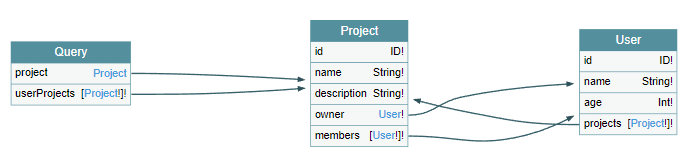
\includegraphics[width=\textwidth,height=\textheight,keepaspectratio]{img/graphqltoy}
    \end{center}
    \caption{Graph des GraphQL-Toys}
    \label{gqltoysschm}
\end{figure}

Entwickelt wurde dieses System mit dem Hintergrund, dass bekannte Bugs im Code eingebracht werden und überprüft werden kann, ob das Testtool diese findet.
Insgesamt wurden 15 verschiedene Bugs eingefügt, welche in verschiedene Kategorien fallen wie Syntaxfehler, falsche Rückgabedaten, falsche Datenstrukturen etc.
Einige der Bugs werden im Folgenden kurz vorgestellt.
Eine Liste aller eingebauten Bugs findet sich im Anhang unter \textit{GraphQL-Toy Implementation mit Bugs}~\ref{graphql-toy-code}.

\subsubsection{Bug 1 - SyntaxFehler}

Diverse Syntaxfehler wurden an verschiedenen Stellen eingebaut.
Dies bedeutet, dass jeder Funktionsaufruf dieser Funktion garantiert scheitern wird.
Somit kann jede Request diesen Fehlerfall entdecken, solange die Request auch das Feld hinter der Funktion mit dem Syntaxfehler abfragt.
Ein einfacher Syntaxfehler findet sich in Listing~\ref{synfe} \\

\begin{lstlisting}[language=javascript, caption={Ein Syntaxfehler}, label={synfe}]
    const resolvers = {
        Query: {
            project: (_, {id}, context, info) => {
                // Example bug 1 - Syntax mistake
                return db.projects.find(project => project.id ===);
            }
        }
    }
\end{lstlisting}

Hierbei fehlt der Wert, mit dem die $project.id$ verglichen werden soll.
Jeder Aufruf dieser Funktion mit egal welcher $ID$ führt zu einem Fehler.

\subsubsection{Bug 2 - Falscher Objekttyp}

Objektfehler sind Fehler, bei denen ein falsches Objekt zurückgegeben wird.
Das Objekt passt dabei nicht zu der definierten Struktur im Schema.
GraphQL wird dann einen Fehler erzeugen, da die Daten nicht zum Schema passen.
Code der zu solch einem Fehler führt ist in Listing~\ref{objfail} dargestellt.

\begin{lstlisting}[language=javascript, caption={Ein Objektfehler}, label={objfail}]
    const resolvers = {
        Query: {
            project: (_, {id}, context, info) => {
                // Example bug 5 - wrong type "error"
                return { ...db.projects.find(project => project.id === id), name: ["a", "b"] };
            }
        }
    }
\end{lstlisting}

Sollte das Feld ein Argument benötigen, so muss dieses passen, sodass auch wirklich ein Objekt abgefragt wird und dann der falsche Type zurückgegeben wird.

\subsubsection{Bug 3 - Typfehler in der Eingabe}

Felder wie $ID$ sind im GraphQL-Standard als einzigartige Strings definiert.
Im Allgemeinen wird der $ID$ Type jedoch von diversen Entwicklern als Zahlenstring genutzt.
Eine Funktion wandelt diesen String dann in eine Zahl, die zum Beispiel genutzt wird, um einen bestimmten Eintrag eines Arrays zu bekommen.
Inputvalidierung wird also benötigt.
In Listing~\ref{ggg} ist Code dargestellt, der zu solch einem Fehler führt.

\begin{lstlisting}[language=javascript, caption={Code ohne Inputvalidierung}, label={ggg}]
    const resolvers = {
        Query: {
            project: (_, {id}, context, info) => {
                // Example bug 3 - Input type validation bug
                return db.projects[id];
            }
        }
    }
\end{lstlisting}

Es ist bei diesem Code möglich, ohne jegliche Prüfung einen Key anzugeben.
Ist ein Resolver so implementiert, dann ist ein IndexOutOfBound Fehler sehr wahrscheinlich.
\\


Mit dem Testtool nach~\cite[Property-based Testing]{property-based-testing} konnten 73\% der Fehler, also 11 der 15 Fehler gefunden  werden.
Der hier entwickelte Prototyp schaffte auf derselben API auch eine Entdeckung von 11 Fehlern.
Es konnte also dieselbe Fehlerfindung erreicht werden.
Mit dem Research-Tool vom Lehrbuch~\cite{software-testing} wurde ermittelt, dass der zugrundeliegende Graph mit PrimePfad Abdeckung 3 Pfade definiert, die es abzudecken gilt.
Diese sind: $. [Query,Project,User]$, $[Project,User,Project]$ und $[User,Project,User]$.
Der Prototyp hat diese erfolgreich erkannt.
Die Generierung der validen GraphQL Anfragen führte zu den Pfaden $[Query, Project, User]$, $[Query, Project, User, Project]$ und $[Query, Project, User, Project, User]$.
Da eine korrekte GraphQL Anfrage stets im Query-Knoten beginnt, ergibt sich, dass die Pfad hier eine ähnliche Struktur zu beginn haben, da diese stets über die Knoten $Query$ und $Project$ laufen müssen.
Bemerkenswert hierbei ist allerdings, dass das Property-based Tool hierfür wesentlich mehr Queries benötigte, um eine zufriedenstellende Coverage zu erreichen.
Das Property-based Tool benötigte 30 Durchläufe, die jeweils bis zu 100\% Kantenabdeckung liefen, um alle Fehler zu finden.
Im Kontrast dazu konnte die hier entwickelte Methode mithilfe von 3 Pfaden eine PrimePfad-Abdeckung erreichen.
Es wurden für jeden Pfad 5 Testquerys entwickelt.
So war es möglich, alle 11 Fehler zu finden.
Bemerkenswert war, dass zwei perfekte Querys ermittelt wurden.
Beide Querys sind in Listing~\ref{q1} und Listing~\ref{q2} gezeigt. \\

\begin{lstlisting}[language=GraphQL, caption={Query 1}, label={q1}]
    { project(id: "2", ) {  id  name  description   owner {  id  name  age   }  }  }
\end{lstlisting}

\begin{lstlisting}[language=GraphQL, caption={Query2}, label={q2}]
    { userProjects(id: "1") { name owner { id name age projects { name description id owner { id name age } } } } }
\end{lstlisting}

Mithilfe dieser Querys kann jeder der 11 entdeckten Fehler gefunden werden.
Dies liegt auch daran, dass der Argumentgenerator entsprechend angepasst wurde und nur valide IDs produziert hat.
So war es sehr wahrscheinlich, dass eine ID, die generiert wird, mindestens in einer der 5 erstellten Querys zur zugrundeliegenden Datenstruktur gepasst hat
und eine tatsächliche Testausführung stattfand und nicht nur ein initialer $null$-Wert, der die Query sofort vorzeitig beendet, zurückgegeben wurde.
Die 4 nicht gefundenen Fehler sind dieselben Fehler wie diese, die \textit{Property-based Testing}~\cite[vgl. RQ.2]{property-based-testing} nicht finden konnte.
Es sind die Felder, in denen ein falscher Wert eines Objektes genutzt wurde, um ein anderes Objekt zu erlangen.
Hierbei verhindert der Black-Box Ansatz, dass der Fehler gefunden wird da eine leere Rückgabe des Feldes eine valide Antwort ist.
Der Black-Box Ansatz limitiert hierbei das Verhalten des Prototypen da dieser nicht genügen Domänenwissen hat, um diesen Fehler zu erkennen.
In diesem Beispiel hat der Prototyp dieselben Fähigkeiten wie der Prototyp von \textit{Property-based Testing}.
Die Ergebnisse der Experimente befinden sich im \href{https://github.com/gernhard1337/GraphQL-Testautomatisierung/tree/main/experiment/toy-experiment}{GitHub}.

\subsection{GitLab}

Das Testsystem GitLab wurde schon in Property-based  Testing verwandt, um an einem Industriereifen Projekt die Methode zu evaluieren~\cite[vgl. Experiment]{property-based-testing}.
Die entwickelte Methode soll sich auch an GitLab beweisen.
GitLab stellt sowohl eine REST als auch GraphQL-API zur Kommunikation  zur  Verfügung.
Mit GitLab wird ein komplexes Softwareprodukt zur Versionsverwaltung und DevOps-Anwendung getestet.
Die Komplexität dieser Software wird deutlich, wenn das GraphQL-Schema von GitLab betrachtet wird, welches in Abbildung~\ref{gitlabschema} zu finden ist.
Eine hochauflösendere Version ist im \href{https://github.com/gernhard1337/GraphQL-Testautomatisierung/blob/main/latex/img/gitlabgraph.png}{GitHub} verfügbar.
Das Schema ist sehr komplex und stark zyklisch.

\begin{figure}[H]
    \begin{center}
        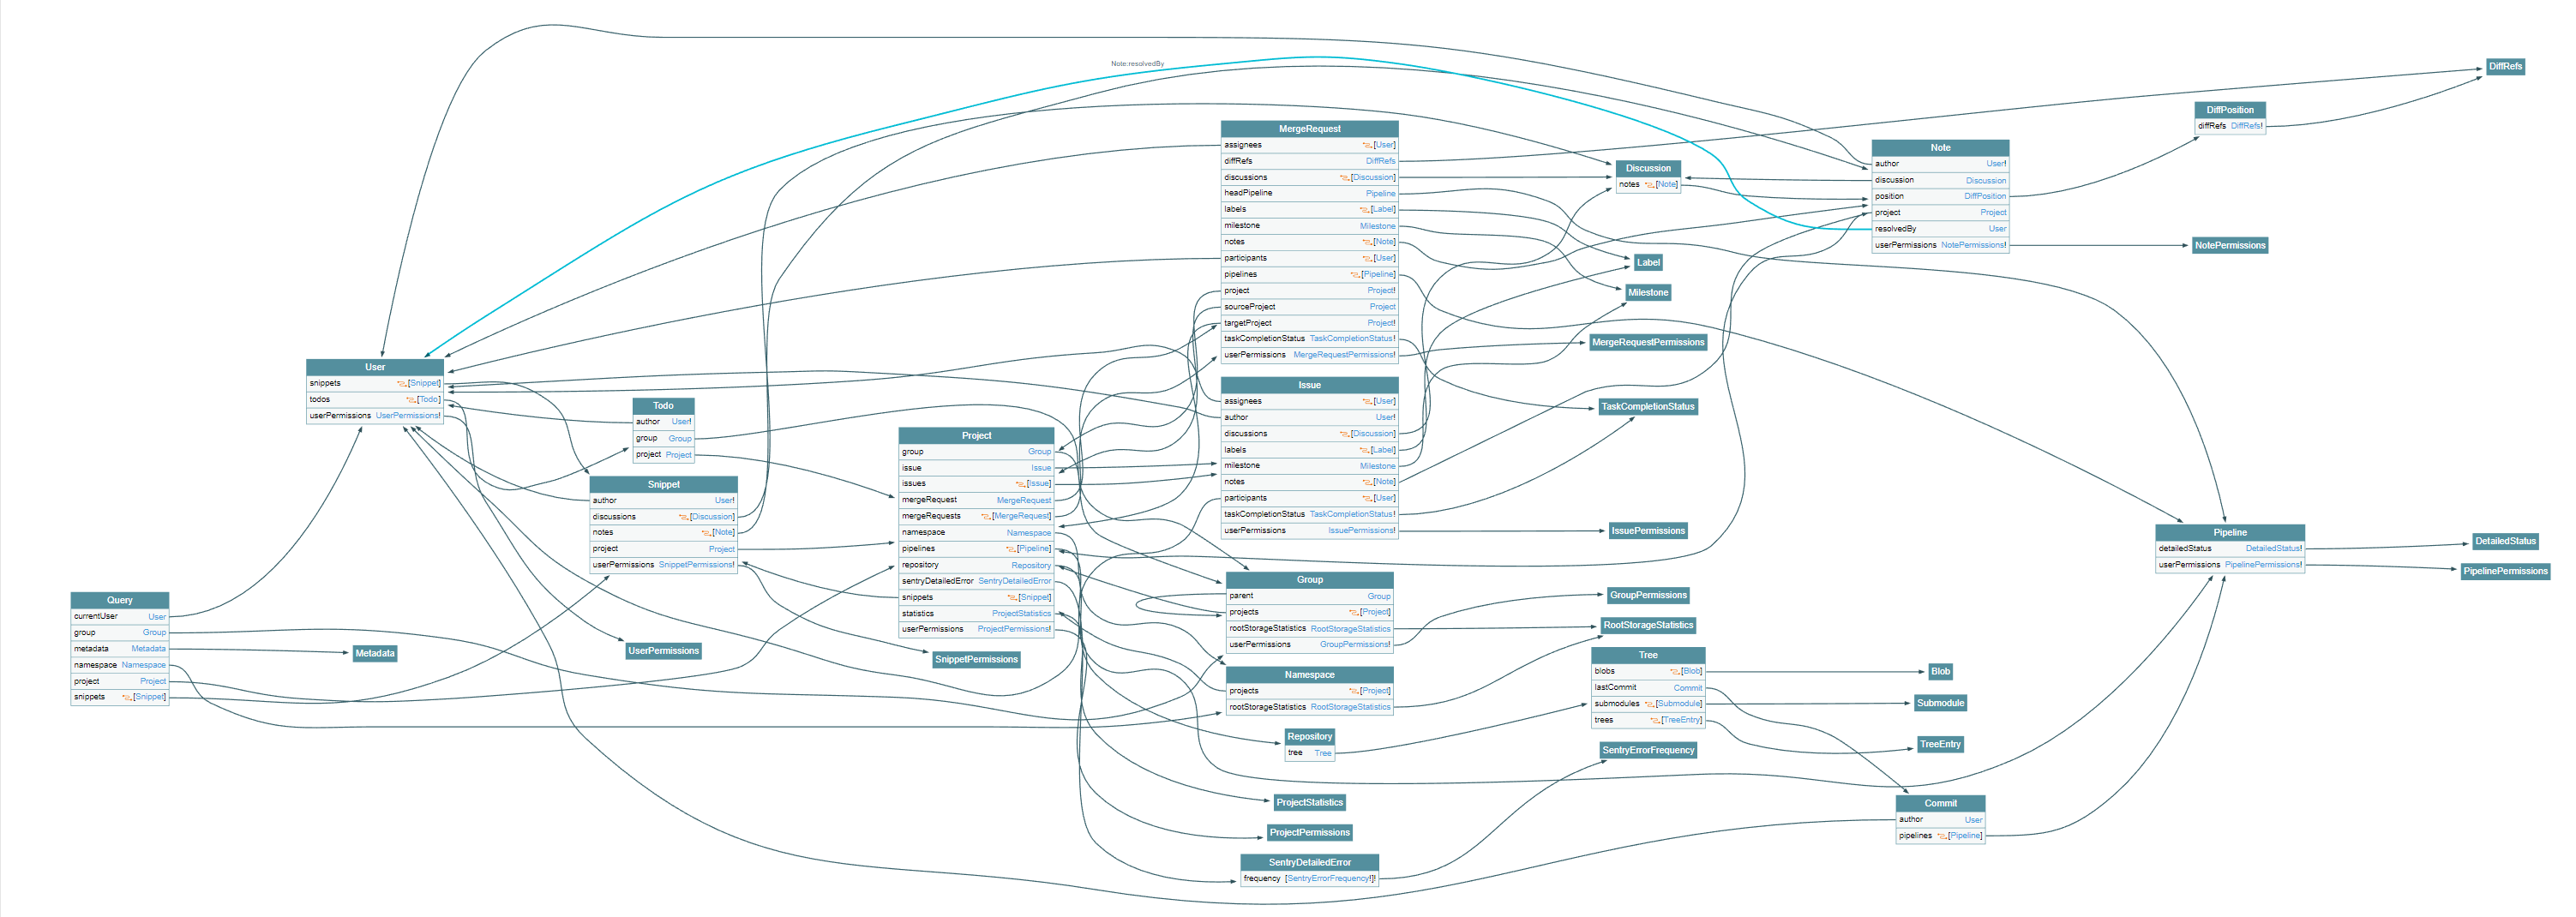
\includegraphics[width=\textwidth,height=\textheight,keepaspectratio]{img/gitlabgraph}
    \end{center}
    \caption{GitLab GraphQL-Schema}
    \label{gitlabschema}
\end{figure}

Das \textit{Property-based Testtool} fand insgesamt 4 Fehler, die im Query-Bereich von GraphQL waren.
Alle Fehler waren Fehler in der Validierung von Eingabevariablen.
Hierbei lag der Fehler darin, dass die Resolver einen Fehler verursachten, wenn als Eingabe ein String mit leerem Zeichen kam.
Dies bedeutet, ein leerer String \verb+""+ wird richtig behandelt (außer in Fehler 4) aber ein String mit leerem Zeichen \verb+e\u0000\+ führt zum Fehler.
Die Fehler wurden gefunden durch die Querys aus Listing~\ref{i1},~\ref{i2},~\ref{i3} und~\ref{i4}.

\begin{lstlisting}[language=GraphQL, caption={Fehler 1\cite{issue1}}, label={i1}]
{project(fullPath: "root/test-project") {sentryDetailedError(id: "") {count}}}
\end{lstlisting}

\begin{lstlisting}[language=GraphQL, caption={Fehler 2\cite{issue2}}, label={i2}]
{project(fullPath: "e\u0000") {name fullPath}}
\end{lstlisting}

\begin{lstlisting}[language=GraphQL, caption={Fehler 3\cite{issue3}}, label={i3}]
{namespace(fullPath: "e\u0000") {fullName name fullPath}}
\end{lstlisting}

\begin{lstlisting}[language=GraphQL, caption={Fehler 4\cite{issue4}}, label={i4}]
{group(fullPath: "e\u0000"){fullName name fullPath }}
\end{lstlisting}

Alle vom \textit{Property-based Testtool} gefunden Fehler wurden durch den hier entwickelten Prototypen ebenfalls gefunden.
Dafür waren die Querys \hyperref[query1]{Query 1}, \hyperref[query2]{Query 2}, \hyperref[query3]{Query 3} und \hyperref[query4]{Query 4} ausreichend.
Es ist zu beobachten, dass die Querys wesentlich länger sind als jene, die vom \textit{Property-based Testtool} erstellt wurden.
Dies liegt an den PrimePfaden, welche die längsten einfachen Pfade darstellen.
Getestet wurde auf dem offiziellen GitLab-Docker Image in der Version 12.6.3
Damit im GitLab auch Daten verfügbar sind, wurde ein Population-Skript geschrieben, das im GitLab
50 User anlegt und jedem User einige Projekte, Commit, MergeRequests etc. zuordnet.
Das Population-Skript kann im~\cite[Github]{populationscript} gefunden werden.
Da die Querygenerierung stets im Query-Knoten beginnt und die PrimePaths gefunden werden sollen, ergeben sich in diesem speziellen Schema sehr viele ähnliche Querys.
Diese unterscheiden sich insbesondere am Ende der jeweiligen Query.
Der zuvor vorgestellte Algorithmus errechnet für das Schema von GitLab eine Pfadanzahl von 41744 für eine PrimePath-Coverage des Schemas.
Eine genaue Auflistung aller Pfade findet sich im~\cite[GitHub]{gitlabpaths}.
Mit der Maßgabe, dass pro Pfad 5 Tests erzeugt werden sollen, wurden dann 208.720 Tests erzeugt.
In nahezu allen Fällen haben die generierten Tests eine tatsächliche Pfadlänge, die kleiner ist als die erwartete.
Dies begründet sich damit, dass an verschiedenen Stellen des Schemas von GitLab Argumente angegeben werden müssen
und mit jedem Argument, das zusätzlich generiert wird, steigt die Wahrscheinlichkeit, dass die zufällige Kombination unpassend ist.
In mehreren Durchläufen zeigte sich, dass im Schnitt nur ungefähr 20 Tests eine ideale Pfadlänge erreichen.
Die Tests, die das Erreichen sind, im Allgemeinen auch Tests, die einen sehr kurzen Pfad abbilden.
Hierbei verringert sich das Risiko, dass Eingabeargumente generiert werden, die keine zugrundeliegenden Daten haben und somit die Pfadausführung verhindern.
Ein Beispiel hierfür ist der Pfad $Query -> Project -> MergeRequest -> Time$.

\begin{lstlisting}[language=GraphQL]
{ project(fullPath: "groupx_3/projectx_2_1") {
    archived
    avatarUrl
    containerRegistryEnabled
    ...
    mergeRequest(iid: "1") {
        allowCollaboration
        createdAt
        mergeStatus
        ...
        }
    }
}
\end{lstlisting}

Durch Anpassen des $FullPath$ Argumentgenerators war es möglich, eine Query zu generieren, die passende Argumente generiert hat, um für eine ideale Testabdeckung (d.h. Länge Ergebnis = Länge Testpfad) zu sorgen.
Generell zeigt sich sehr schnell, dass bei der hier entwickelten Methode ähnliche Limitierungen wie im Property-based Testing auftreten.
So ist eine manuelle Anpassung der Argumentgeneratoren an das Domänenwissen nötig.
Für GitLab bedeutet dies unter anderem, dass die ID-Struktur, um zum Beispiel Projekte abzufragen, in der Form \verb+<user>/<project>+ sein muss~\cite[vgl. S.8]{property-based-testing}.
Da hier ähnliche Argumentgeneratoren verwendet wurden wie in Property-based Testing, leiden diese unter derselben Limitierung des mangelnden Domänenwissens~\cite[vgl. S.8]{property-based-testing}.
Es werden zwar sehr viele Tests entwickelt, die die PrimePfad Abdeckung umsetzen.
Wenn jedoch die Generierung der Tests auf Zufall basiert, so kann nicht garantiert werden, dass die Eingabeargumente passend sind und ein valides Ergebnis zurückgeben.
Wird kein Ergebnis zurückgegeben, so folgert GraphQL, dass spätere Funktionen nicht ausgeführt werden müssen und somit werden diese auch nicht getestet.
Es ist möglich, dieses Problem zu beheben, hierzu jedoch in Kapitel~\ref{futurework} mehr.

\section{Schema-Abdeckung}

Wie in Property-based Testing schon erwähnt: \textit{da keine Coverage Metric für GraphQL Blackbox Test Auswertung existiert, starten wir mit einem sehr
einfachen und intuitiven Ansatz}~\cite[vgl. B. Measuring Schema Coverage]{property-based-testing}.
Das in \textit{Property-based Testing} vorgestellte Abdeckungskriterium ist die Kantenabdeckung, wie schon in Abschnitt~\ref{propiskant} gezeigt.
Da jedoch das Rekursionslimit die Pfadlänge begrenzt, wird der Graph des Schemas künstlich beschnitten und alle Pfade, die länger als
das Rekursionslimit sind, werden in der Abdeckung nicht berücksichtigt.
Hierdurch folgt, dass sich die gewünschte Kantenabdeckung in Realität nicht zuverlässig ergibt, da GraphQL-Schemas durchaus Pfadlängen länger
als das Rekursionslimit zulassen (das Rekursionslimit wurde standardmäßig auf 4 gesetzt~\cite[vgl. SourceCode ]{property-based-testing}).
Um die gewünschte Kantenabdeckung zu erreichen, musste im \textit{Property-based Testing} außerdem die Generierung mehrfach ausgeführt werden, bis die Abdeckung erreicht wurde.
Um eine vollständige Abdeckung beim GitLab Schema zu erreichen, waren diverse Iterationen nötig bei verschiedenen Rekursionslimits.
Eine 100\% Coverage wurde bei GitLab nur in einem Versuch erreicht, wenn 10000 Tests mit Rekursionslimit 4 erstellt wurden~\cite[vgl. Tabelle 2]{property-based-testing}.
Da der Graph des GitLab-Schemas jedoch beschnitten wurde, da dieser, wie später gezeigt wird, wesentlich größer ist, kann nicht gesagt werden, dass vollständige Kantenabdeckung erreicht wurde.
Der wesentliche Unterschied beider Methoden ist, dass \textit{Property-based Testing} Experimente für die theoretische Abdeckung ausführen muss
und hierbei werden mehrere Iterationen benötigt, um diese zu erreichen.
Der Ansatz der PrimePfad-Abdeckung im hier entwickelten Prototypen stellt sicher, dass die generierten Pfade PrimePfade sind.
Somit ist zugesichert, dass die Abdeckung erfüllt ist.
Die PrimePfad Abdeckung wird auf unbeschnittenen Graphen ausgeführt und ist auch im Allgemeinen ein stärkeres Kriterium nach Definition~\ref{sort}.
Es kann also gefolgert werden, dass die hier entwickelte Methode eine Verbesserung der theoretischen Abdeckung erzielt hat.
Ein praktischer Nachweis hierfür folgt in den nächsten Abschnitten.
Die Limitierung der zufälligen Argumentgeneratoren behindert eine tatsächliche Umsetzung der theoretischen Abdeckung.
Allerdings ist diese Limitierung potenziell lösbar, hierzu in Kapitel~\ref{futurework} mehr.
\newpage

\subsection{GraphQL-Toy Schema Coverage}

Wie eingeführt in \textit{Property-based Testing}~\cite{property-based-testing} muss für eine zufriedenstellende Abdeckung
die Defintion~\ref{defedgecov} erfüllt sein, dass jedes Paar von \verb+(Type, objectField)+ berücksichtigt ist.
Dies bedeutet für das Schema, dass die folgenden Tupel abgedeckt sein müssen, um Kantenabdeckung zu erfüllen.
    \begin{itemize}
        \item \verb+(Query, project)+
        \item \verb+(Query, userProject)+
        \item \verb+(Project, owner)+
        \item \verb+(Project, members)+
        \item \verb+(User, projects)+
    \end{itemize}

Da nur die beiden initialen Felder aus dem Query-Type Eingabeargumente benötigen, ist die Querygenerierung simpel.
Es kann keine Aussage darüber gemacht werden, ob die generierten Querys von \textit{Property-based Testing}~\cite{property-based-testing} diese Abdeckung erfüllen, denn bei der Querygenerierung spielt es keine Rolle, ob dieses Kriterium erreicht wird.
Es gibt lediglich eine Messung die zeigt, dass der Prototyp mit hinreichender Wahrscheinlichkeit in der Lage ist, durch zufällige Querygenerierung Tests zu generieren, die Kantenabdeckung erfüllen~\cite[vgl. D.Results RQ1 ]{property-based-testing}.
Im Gegensatz zum Property-based Testing hat der hier entwickelte Prototyp den Vorteil, dass die Pfadgenerierung nicht zufällig ist.
Dadurch ergibt sich, dass die Tests, die vom hier entwickelten Prototyp aufgrund eines stärkeren Abdeckungskriteriums erstellt werden, stets auch die Kantenabdeckung erfüllen.
Ein einziger Durchlauf reicht aus, um sicherzustellen, dass die gewünschte Abdeckung zumindest theoretisch erreicht ist.
Natürlich bleibt offen, ob die generierten Tests diese Coverage tatsächlich erreichen jedoch ist dies auch ein Problem im \textit{Property-based Testing}.
Dort wird nur geprüft, ob die Felder in der Anfrage existieren jedoch nicht, ob die Antwort diese auch enthält.
Um dies messbar zu machen wurde zuvor die Abschätzund der Pfadlängen eingeführt.
Hierdurch konnte gezeigt werden, dass die generierten Querys in Teilen die Abdeckung auch tatsächlich umsetzen.

\subsection{GitLab Schema Coverage}

Das GitLab Schema ist wesentlich komplexer und zyklischer als das GraphQL-Toy.
Im Gegensatz zum GraphQL-Toy besteht das GitLab Schema aus 37 Knoten, welche jeweils zahlreiche Kanten hinzufügen.
Generell lässt sich sagen, dass das Schema sehr komplex und stark rekursiv ist~\cite[vgl. Studied Cases 2]{property-based-testing}.
Da der Property-based Testing Ansatz ein Rekursionslimit benötigt stellt, sich die Frage inwiefern überhaupt dieses Schema überdeckt werden kann.
Laut Paper hat sich ein Rekursionslimit von vier als hinreichend ausgezeichnet~\cite[vgl. Table 1 ]{property-based-testing} und wurde auch so im Code übernommen.
Ein Rekusionslimit von vier bedeutet, dass die maximale zu erreichende Pfadlänge des Testpfades vier ist.
Da das GitLab-Schema aber einen Graphen aufspannt, der durchaus wesentlich längere Pfade als vier hat, ist es fragwürdig wie die 100\% Schema-Coverage in~\cite[Table 1]{property-based-testing} berechnet wurde.
Es seien hier einige Pfade beispielhaft genannt, die einzigartig sind, bei denen sich keine Kante doppelt und deren Länge 4 stark überschreitet: \\

\begin{itemize}
    \item Query \textrightarrow User \textrightarrow SnippetConnection \textrightarrow SnippetEdge \textrightarrow Snippet \textrightarrow DiscussionConnection \textrightarrow DiscussionEdge \textrightarrow Discussion \textrightarrow NoteConnection \textrightarrow NoteEdge \textrightarrow Note \textrightarrow Project \textrightarrow IssueConnection \textrightarrow Issue \textrightarrow Milestone \textrightarrow Time
    \item Query \textrightarrow Project \textrightarrow Issue \textrightarrow DiscussionConnection \textrightarrow DiscussionEdge \textrightarrow Discussion \textrightarrow NoteConnection \textrightarrow NoteEdge \textrightarrow Note \textrightarrow User \textrightarrow SnippetConnection \textrightarrow SnippetEdge \textrightarrow Snippet \textrightarrow Time \\
    \item Query \textrightarrow Namespace \textrightarrow ProjectConnection \textrightarrow Project \textrightarrow MergeRequestConnection \textrightarrow MergeRequestEdge \textrightarrow MergeRequest \textrightarrow UserConnection \textrightarrow User \textrightarrow SnippetConnection \textrightarrow Snippet \textrightarrow DiscussionConnection \textrightarrow PageInfo \\
\end{itemize}

Durch die Beschneidung des Graphens in \textit{Property-based Testing} durch das Rekursionslimit folgt, dass die ermittelte Kantenabdeckung
nicht zutreffend ist und nur für einen Teilgraphen des gesamten Graphens zutrifft.
Dies ist ein sehr großer, struktureller Einschnitt und die in Property-based Testing genannten 100\% Kantenabdeckung ist keine tatsächliche Kantenabdeckung,
sondern eben nur für den abgeschnittenen Teilgraphen.
Wie zuvor gezeigt, erzeugt der hier entwickelte Prototyp Tests, die PrimePfad-Abdeckung umsetzen und somit ein stärkeres Abdeckungskriterium erfüllen.
Eine komplette Pfadgenerierung auf dem gesamten Graphen hatte als Ergebnis, dass über 40.000 Pfade benötigt werden, um eine PrimePfad-Abdeckung für das GitLab-Schema zu erreichen.
Hier zeigt sich auch ein direkter Unterschied.
Während in Property-based Testing gesagt wird, dass 10.000 Tests mit einem Rekursionslimit von 4 ausreichen, um eine vollständige Kantenabdeckung zu erreichen~\cite[vgl. Table 1]{property-based-testing}
so wurde gezeigt, dass 10.000 Tests nicht ausreichen können, wenn allein über 40.000 PrimePfade existieren.
Die Berechnung der Querys geschah auf einem hardwaretechnisch ähnlichem Level wie in Property-based Testing verwandt~\cite[vgl. Experimental Setup]{property-based-testing}.
Hier wurde die Aussage getroffen, dass ein~\textit{Tiefensuchen Ansatz nicht skaliert und deswegen ein iterativer Ansatz zu präferieren ist}~\cite{property-based-testing}.
Der hier entwickelte Prototyp zeigt das Gegenteil.

\section{Zusammenfassung der Experimente}

Mit den beiden Experimenten konnte gezeigt werden, dass der Prototyp dieselben Fehler findet wie der Prototyp aus Property-based Testing.
Es wurde gezeigt, dass die theoretische Abdeckung eines GraphQL-Schemas mit dem Prototypen immens gesteigert wird ohne,
wie in~\cite{property-based-testing} behauptet, die Berechnungszeit signifikant zu erhöhen.
Während die theoretische Abdeckung des Graphens erhöht wurde, so zeigte sich, dass die reale Abdeckung nicht mit der theoretischen Abdeckung mithalten kann.
Die Pfadlänge der generierten PrimePfade ist im Allgemeinen sehr lang und hierdurch steigt die Wahrscheinlichkeit, dass ein Pfad nicht komplett ausgeführt wird.
Eine Anpassung der Argumentgeneratoren an das jeweilige SUT ist sinnvoll und verbessert die Pfadlängen der Tests.
Das mangelnde Domänenwissen limitiert die Resolver in derselben Weise wie im \textit{Property-based Testing} wo es heißt: wo es heißt:
\textit{.. das Domänenwissen von zugrundeliegenden Entitäten eine stärkere Testumgebung erzeugen kann}~\cite[S.8]{property-based-testing}.
Möglichkeiten, um das Domänenwissen über das SUT zu erhöhen, werden in Kapitel~\ref{futurework} vorgestellt.
